\subsection{Blobs}
En blob er en region i et billede, hvor intensitet er konstant, og forskellig fra intensiteten udenfor regionen. Lindenberg \cite{blob} definere blobs som værende lyse regioner på sort baggrund eller omvendt - altså strukturer, der står i kontrast til deres baggrund. 

%Det lokale ekstrema gør blobben til en veldefineret, lav-niveau struktur og kravet om konstant intensitet gør den pr. definition distinktiv. 
\begin{figure}[H]
    \centering
    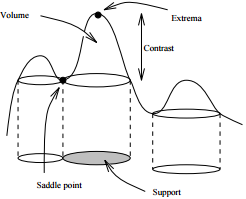
\includegraphics[width=0.35\textwidth]{fig/11.png}
    \vspace{-0.5em}   
    \begin{center}
    \caption{\textcolor{gray}{\footnotesize \textit{
    En blob visualiseret i 2-d, udefra Lindenberg's definition \cite{blob}}}}
    \label{fig:lindblob}
     \end{center}
  \end{figure}
       \vspace{-2.7em}
\noindent
I figur \ref{fig:lindblob}(a), ses en blob defineret af dens lokale ekstrema, hvor styrken af blobben beksrives ved kontrasten, ift. området omkring ekstremaet. Lindenberg definere en blob som værende afgrænset af dens saddelpunkt; et saddelpunkt angiver punktet, hvor intensiteten stopper med at falde og starter med at stige for lyse blobs, og modsat for mørke.
\\
\\
En metode til at detektere ekstremaer, er Laplace af Gauss(LoG). Laplace defineres således:
\begin{equation}
\Delta f = \nabla^2 f =  \sum_{i = 1}^n \frac{\partial^2 f}{\partial x^2_i}
\end{equation}
Anvendes Laplace operatoren på gaussfunktionen ligning \eqref{2dgaussian}, kan der dannes en kerne, der fremhæver regioner, som beskrevet. 
\begin{equation}
LoG= \sigma^2\Delta G
\label{lap}
\end{equation}
Bemærk, at $\sigma^2$ er blevet multipliceret på fra venstre. Dette er gjort for at normalisere LoG, således, at responset er invariant overfor størrelsen af $\sigma$. LoG kan diskritiseres og foldes med billedet for at finde lokale ekstremaer. \\

\begin{figure}[H]
    \centering
    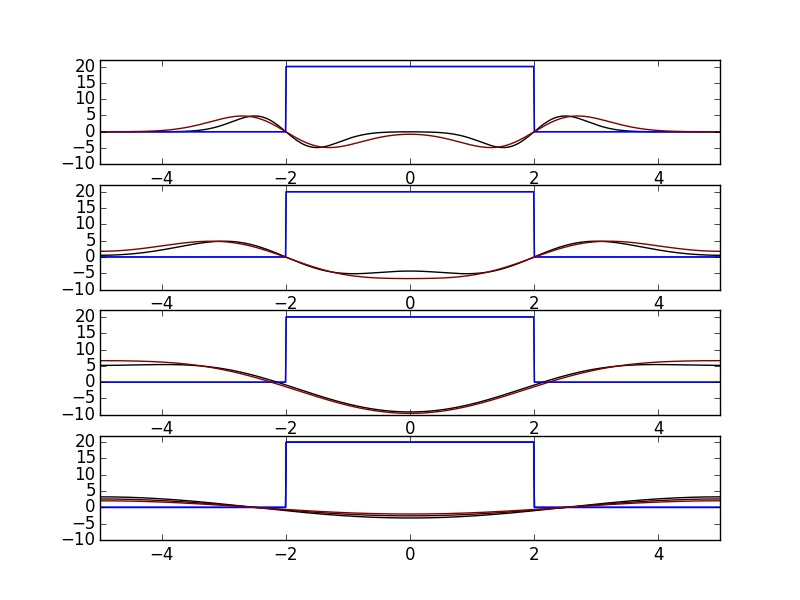
\includegraphics[width=0.90\textwidth]{fig/normLoG.jpg}
    \vspace{-0.5em}   
    \begin{center}
    \caption{\textcolor{gray}{\footnotesize \textit{
    (a) En 3-D visualisering af en to-dimensional Laplacian of Guassian (b) ét en-dimensionalt signal (c) Laplacian of Gaussian operatoren anvendt på (b)}}}
    \label{fig:normLoG}
     \end{center}
  \end{figure}
       \vspace{-2.5em}
\noindent
Et andet problem opstår, når der skal findes en blob. Problemet er illustreret på figur \eqref{fig:normLoG} - hvilke størrelse skal $\sigma$ være, for at finde blobben? Figuren viser fire forskellige værdier for $\sigma$. I første illustration er $\sigma$ værdien for lav - her dannes flere ekstremaer, men ingen af dem karakteriserer et blob, da den absolutte værdi for funktionen evalueret på det afledte af LoG signalet, er for lav. Dog ser illustration tres kurve ud til, at have tilstrækkelig høj absolut værdi, til at kunne karakteriseres som et blob. \\
Problemet omkring valg af skala, kan afhjælpes ved skalarumsrepræsentation, som gennemgås i.

\begin{figure}[H]
    \centering
    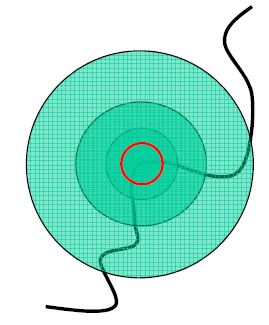
\includegraphics[width=0.25\textwidth]{fig/29.png}
    \vspace{-0.5em}   
    \begin{center}
    \caption{\textcolor{gray}{\footnotesize \textit{
    }}}
    \label{fig:scale}
     \end{center}
  \end{figure}
       \vspace{-2.5em}
\noindent
I figur \ref{fig:scale} angiver cirklerne forskellige undersøgte skalaer, Så hvordan udvælges cirklen, der dækker interesse området uafhængigt af områdets størrelse?  For Blobs er det interessant når der i et skaleret område opstår et veldefineret ekstrema. En måde at søge efter ekstremaer over forskellige skalaer er ved at oprette et skalarum for det undersøgte billede, hvor hvert billede skaleres og der for hver skala findes interessepunkter. Skala-rummet i et 2-dimensionalt billede repræsenteres af flere billeder i forskellige skalaer af det originale billede. Billeder, der repræsentere forskellige skalaer, opnås ved at folde billedet iterativt med et Gaussisk filter med stigende $\sigma$ værdi. 
\begin{figure}[H]
    \centering
    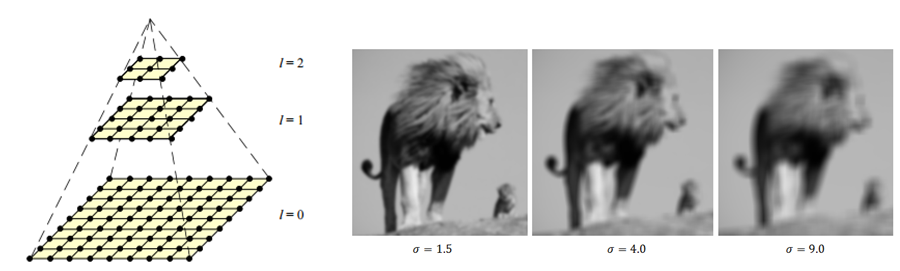
\includegraphics[width=0.65\textwidth]{fig/24.png}
    \vspace{-0.5em}   
    \begin{center}
    \caption{\textcolor{gray}{\footnotesize \textit{
Til venstre ses en visualisering af et skala-rum formet som en pyramide. Hvert niveau angiver en skala repræsentation af det originale vindue, hvor toppen af pyramiden indeholder billeder af største skala og derfor med mindst information, og bunden af skalaen med det originale billede. Til højre ses et billede foldet med et Gaussisk filter af stigende sigma værdier. Jo højere sigma værdi, jo flere fine detaljer bliver fjerne og billedet slørret.
    }}}
    \label{fig:mona}
     \end{center}
  \end{figure}
       \vspace{-2.5em}
\noindent
Et Gaussisk filter bruges da gradvis højere værdier af $\sigma$ fjerner fine strukturer, som vist i figur \ref{fig:mona}, og nye strukturer forekommer ikke ved transformationen fra finere til grovere skalaer \cite{lindenscale}. Idéen er derved at fjerne disse strukturer og lede efter  andre ekstremaer, gradvist på større skalaer, der også kan detekteres.
Et billede i skalarummet for billedet $f(x,y)$ kan derfor defineres som i \eqref{scalespace}
\begin{equation}
L(x,y,\sigma) = G(x,y,\sigma)\ast f(x,y)
\label{scalespace}
\end{equation}
hvor $G$ er det 2-dimensionelle Gaussiske filter,$L(x,y,\sigma)$ repræsentere et et billede i skala-rummet, og skala-parametren $\sigma$, bestemmer skalaen, eller placeringen i skala-rummet. $L(x,y,0) = f(x,y)$, da det er den "nederste" skala og den nederste del af pyramiden. Højere niveauer af pyramiden kan opnås ved at folde billedet med et Gaussisk filter af større sigma værdi.